\documentclass[main]{subfiles}


\title[Tabular Foundation Models]{Tabular Foundation Models}
\subtitle{Pre-Training Allowing to Skip Training}
\author[Marius Lindauer]{Marius Lindauer}
\date{}

\titlebackground*{images/AutoML_Agentic}

%\institute{}
%\date{}

\begin{document}
	
	\maketitle
	

%----------------------------------------------------------------------
%----------------------------------------------------------------------
\begin{frame}[c]{Idea of Tabular Foundation Models}

\begin{itemize}
    \item Traditionally, we train one model for one task on a given dataset
    \item Therefore, we need to find the best hyperparameters, architectures and so on over and over again
    \item But what if we could avoid training models altogether?
    \item Main idea: Pre-train a (tabular) foundation model and only use in-context learning (ICL) on a new dataset
\end{itemize}

$\leadsto$ We will focus on likely the most famous tabular foundation model as of 2026: TabPFN

Other tabular foundation models include TabICL~\liturl{Qu et al. 2025}{https://arxiv.org/abs/2502.05564}\liturl{Qu et al. 2026}{https://arxiv.org/abs/2602.11139} or TabDPT~\liturl{Ma et al. 2024}{https://arxiv.org/abs/2410.18164}.

\end{frame}
%-----------------------------------------------------------------------
%----------------------------------------------------------------------
\begin{frame}[c]{TabPFN: Pre-Training\newline\liturl{Hollmann et. 2022}{https://arxiv.org/abs/2207.01848} \liturl{Hollmann et al. 2024}{https://www.nature.com/articles/s41586-024-08328-6}}

\centering
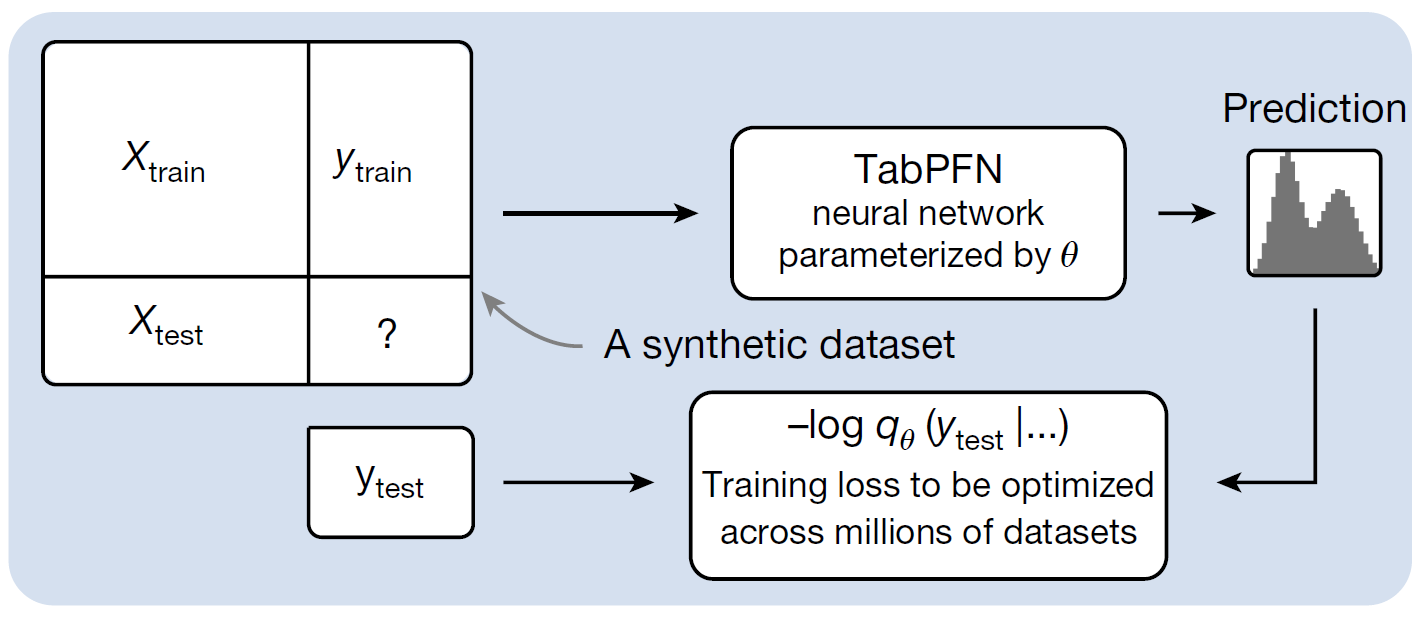
\includegraphics[width=0.8\textwidth]{images/tabpfn_pretraining}

\end{frame}
%-----------------------------------------------------------------------
%----------------------------------------------------------------------
\begin{frame}[c]{TabPFN: Synthetic Data Generation\newline\liturl{Hollmann et. 2022}{https://arxiv.org/abs/2207.01848} \liturl{Hollmann et al. 2024}{https://www.nature.com/articles/s41586-024-08328-6}}

\centering
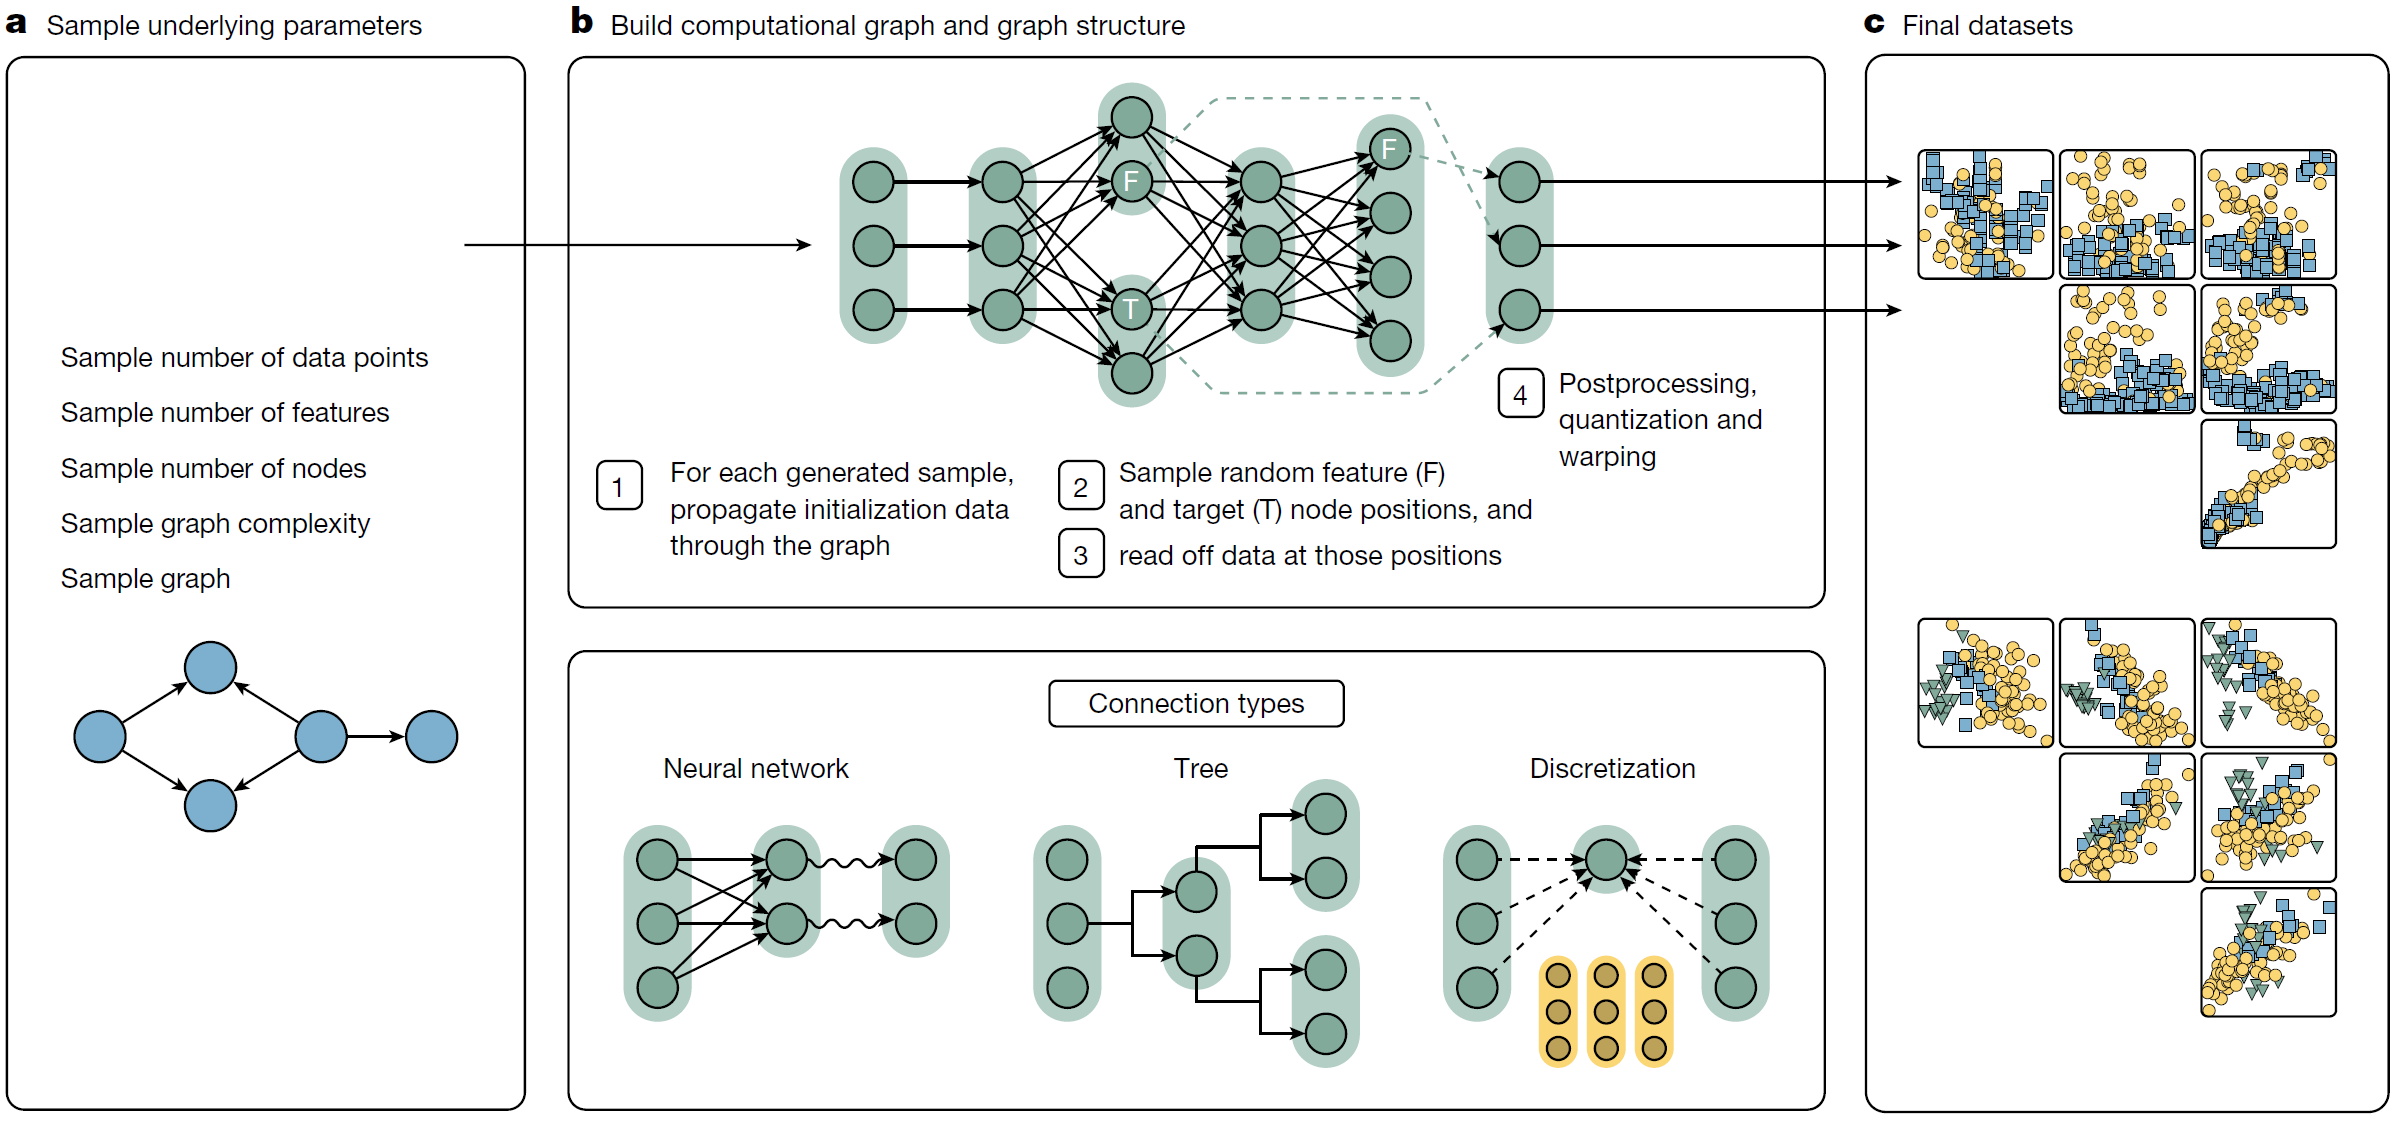
\includegraphics[width=0.9\textwidth]{images/tabpfn_datagen}

\end{frame}
%-----------------------------------------------------------------------
%----------------------------------------------------------------------
\begin{frame}[c]{TabPFN: Prediction\newline\liturl{Hollmann et. 2022}{https://arxiv.org/abs/2207.01848} \liturl{Hollmann et al. 2024}{https://www.nature.com/articles/s41586-024-08328-6}}

\centering
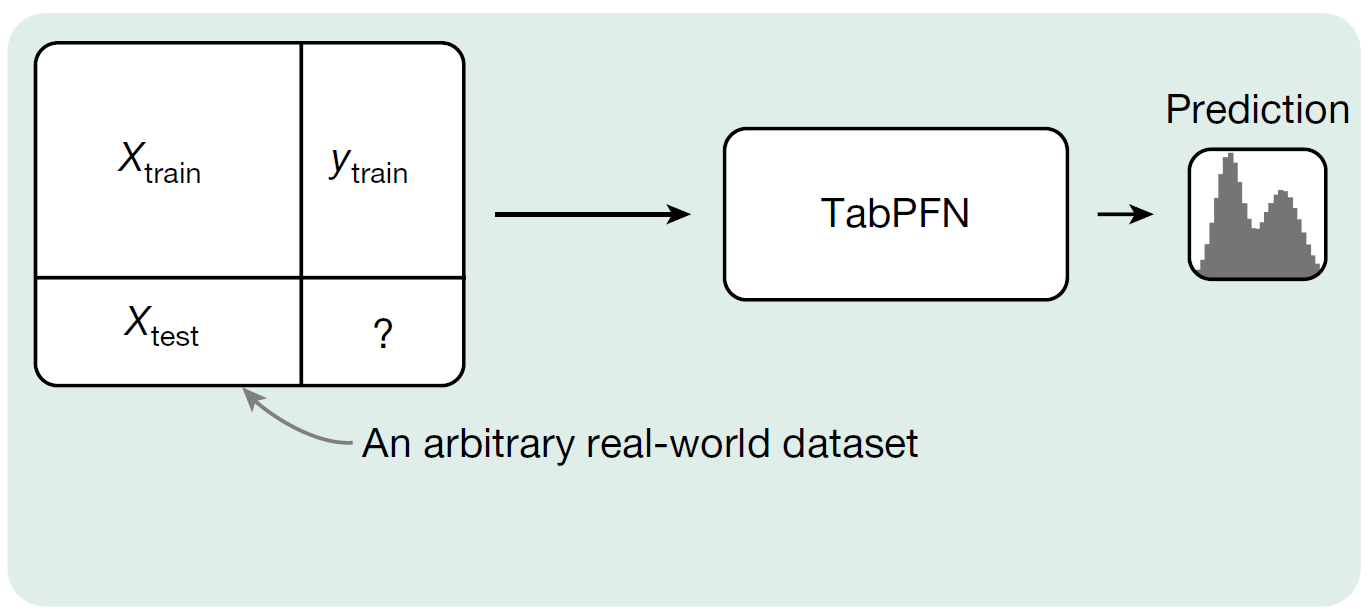
\includegraphics[width=0.8\textwidth]{images/tabpfn_pred}

\end{frame}
%-----------------------------------------------------------------------
%----------------------------------------------------------------------
\begin{frame}[c]{TabPFN: In-Context Learning\newline\liturl{Hollmann et. 2022}{https://arxiv.org/abs/2207.01848} \liturl{Hollmann et al. 2024}{https://www.nature.com/articles/s41586-024-08328-6}}

\centering
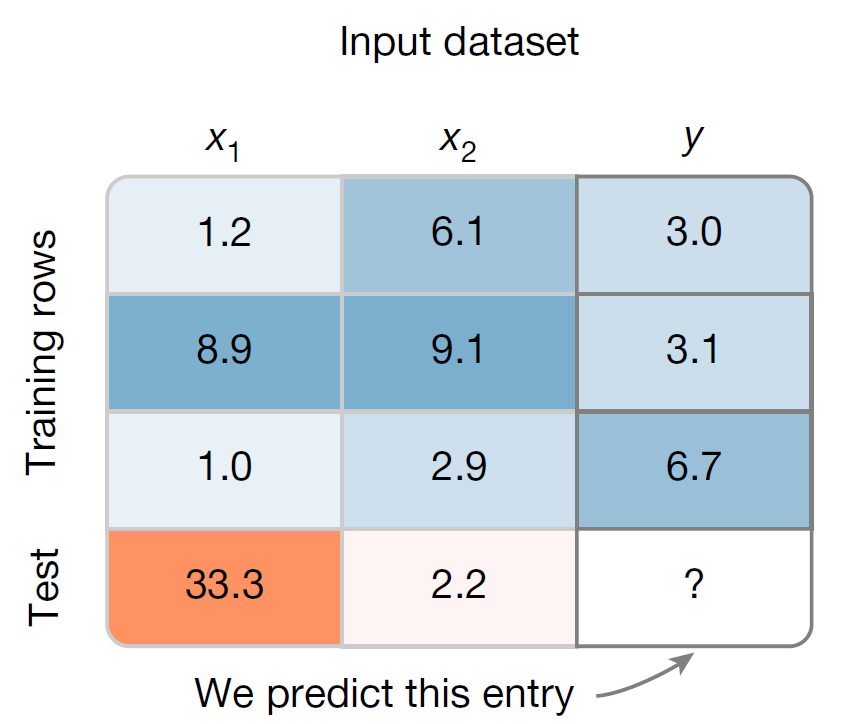
\includegraphics[width=0.5\textwidth]{images/tabpfn_input}

\end{frame}
%-----------------------------------------------------------------------
%----------------------------------------------------------------------
\begin{frame}[c]{TabPFN: In-Context Learning Cont'd\newline\liturl{Hollmann et. 2022}{https://arxiv.org/abs/2207.01848} \liturl{Hollmann et al. 2024}{https://www.nature.com/articles/s41586-024-08328-6}}

\centering
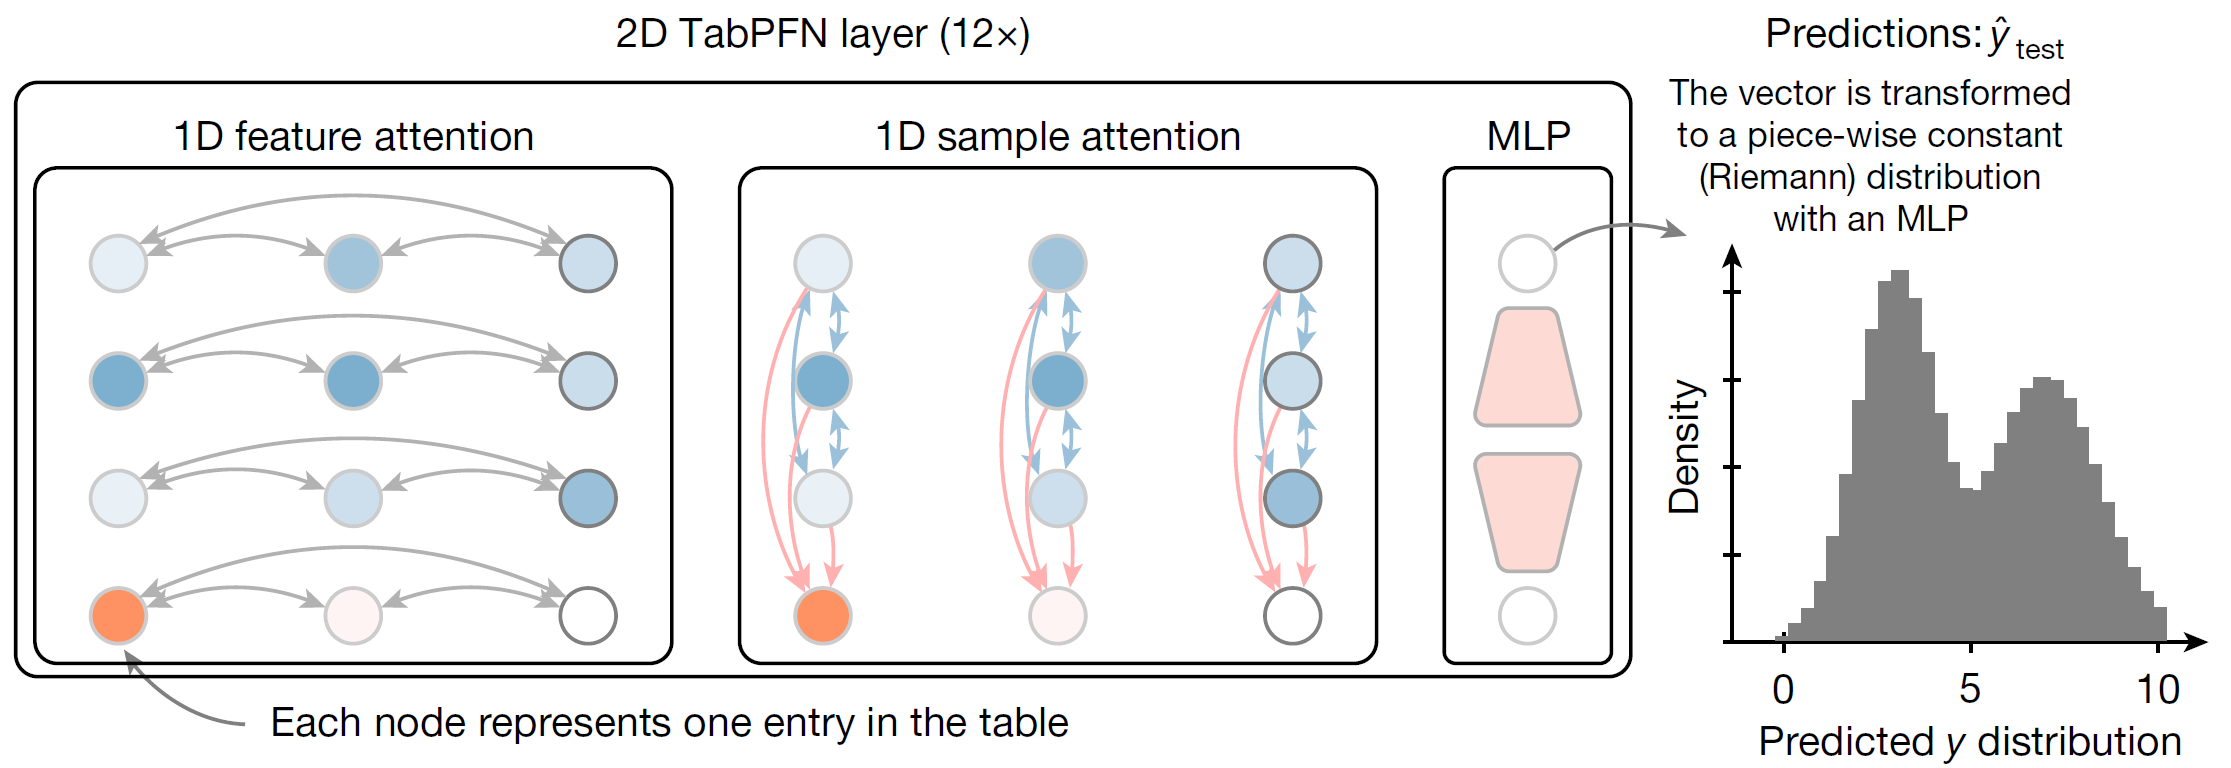
\includegraphics[width=0.9\textwidth]{images/tabpfn_pred2}

\end{frame}
%-----------------------------------------------------------------------

%----------------------------------------------------------------------
\begin{frame}{Summary} 

Most important insights from this video:

\begin{enumerate}
    \item Tabular Foundation Models allow to use a single model for many different datasets
    \item Crucial step is the synthetic data generation process which needs to (sufficiently) resemble real-world data
    \item In-Context-Learning (ICL) allows to feed in an entire dataset (training and test set) and obtain test predictions
\end{enumerate}


\end{frame}

\end{document}

